\section{Processamento da cena do \textit{Freecad}}
Para se iniciar a resolver o problema, é necessário processar os objetos da cena do \textit{FreeCad}, assim permitindo a mineração dos dados destes objetos.

Para o problema de encontrar o empacotar em um retângulo de menor área, referido na seção \ref{cap:introducao:sec:problema}, deve-se seguir a logica abaixo:
\begin{enumerate}
    \item Minimização de altura: Rotaciona os objetos para que as suas faces estejam no plano Z = 0, e que a altura do objeto seja minimizada;
    \item Posição inicial: Reposiciona os objetos em uma posição inicial onde os seus vértices nas coordenadas XY, tenham os seus valores máximos no zero, o motivo, se dá ao fato que o algoritmo genético irá somar a translação destes objetos;
    \item Coleta dos vértices: Será coletado os vértices de cada objeto da cena, e estes serão enviados para o código de \textit{C++}, este irá pre-processar os dados dos vértices, processar o \textit{GA} enquanto salva a performance;
    \item : Será coletado os vértices de cada objeto da cena, e estes serão enviados para o código do \textit{GA}, este irá pre-processar os dados dos vértices, processar o \textit{GA} enquanto salva a performance.
\end{enumerate}

Para o caso de \textit{Knolling}, deve-se adicionar os seguintes passos antes de passar os dados para o código do \textit{C++}:
\begin{enumerate}
    \item Posicionamento da bandeja: Reposiciona a bandeja para que os vértices de menor valor X e Y estejam posicionados no zero;
    \item Coleta dos vértices da bandeja: Se coleta os vértices da bandeja para se usar no \textit{GA}.
\end{enumerate}

\subsection{Minimização da altura}
Para se alocar os objetos em uma bandeja de impressão 3D, se é interessante limitar a altura desses objetos.\newline
Com o intuito de minimizar a altura dos objetos foi feito uma função, com a logica abaixo: 
\begin{enumerate}
    \item Realiza um \textit{loop} por todos os objetos da cena do tipo ``<class `PartDesign.Body'>" e que não possuam o nome "Board Body", pois este está reservado para a bandeja;
    \begin{enumerate}
        \item Realiza um \textit{loop} por todas as faces
        \begin{enumerate}
            \item Onde se verifica a distância de todos os vértices;
            \item Caso essa distância seja menor que a menor altura registrada, esta face será a nova melhor;
        \end{enumerate}
        \item Ao se determinar a melhor face, se determina o vetor normal dessa face;
        \item Partindo desse valor é possível determinar o eixo de rotação e o angulo, assim se determinando o "\textit{spin}";
        \item Ao rotacionar o objeto, se é necessário se determinar a altura do vértice mais baixo, este provavelmente será qualquer vértice da face encontrada, mas foi decidido verificar todos, pois esse pre-processamento não é significativo para o tempo de execução;
        \item Usa a altura do vértice de menor valor em Z para desloca-lo para o plano Z = 0, assim demostrado na figura \ref{fig:Cap03_FreeCad_Rotation}.
    \end{enumerate}
\end{enumerate}

A função "\textit{Rotate2ShorterstHeight}" do \cite{code:FreeCad_Miner}, pode ser encontrada abaixo:

\begin{lstlisting}[language=Python, breaklines, caption = \textit{Rotate2ShorterstHeight}, captionpos=b]
def Rotate2ShorterstHeight( objs ):
    for obj in objs:
        if 'Shape' in dir(obj):
            if str(type(obj)) == "<class 'PartDesign.Body'>" and obj.Label != "Board Body":
                s = obj.Shape
                p = obj.Placement
                b = p.Base
                faces = s.Faces
                size_list = len(faces)
                best_face = -1
                smallest_height = 9999999

                #Look through object faces, looking for the 
                #one which on the bottom would gives us the shortest height
                for i in range( size_list ):
                    height = -1
                    for j in range( size_list ):
                        if i == j:
                            continue
                        for vertex in faces[j].Vertexes:
                            distance = faces[i].distToShape( vertex )[0]
                            if height < distance:
                                height = distance
                    print( "height = ", height )
                    if height < smallest_height:
                        smallest_height = height
                        best_face = i

                #Find Axis and angle to rotate
                uv = faces[ best_face ].Surface.parameter(faces[ best_face ].CenterOfMass)
                faceNormalInCOM = faces[ best_face ].normalAt(uv[0], uv[1])
                angle = acos( -faceNormalInCOM[2] )*180/(pi)

                # Make rotaion, so that face is on the bottom, and orthogonal to XY
                spin = makeRotatingPlacement(App.Vector(b[0], b[1], b[2]), App.Vector(-faceNormalInCOM[1], faceNormalInCOM[0], 0), angle)
                obj.Placement = spin.multiply(obj.Placement)

                #After rotation, sets find lowest high and sets it on zero
                s = obj.Shape
                p = obj.Placement
                b = p.Base
                r = p.Rotation
                lowest_height = 9999999
                for vertex in s.Vertexes:
                    Point = vertex.Point
                    if lowest_height > Point[2]:
                        lowest_height = Point[2]

                obj.Placement = App.Placement(App.Vector(b[0], b[1], b[2] - lowest_height), r)
\end{lstlisting}

\begin{figure}[H]
    \centering
    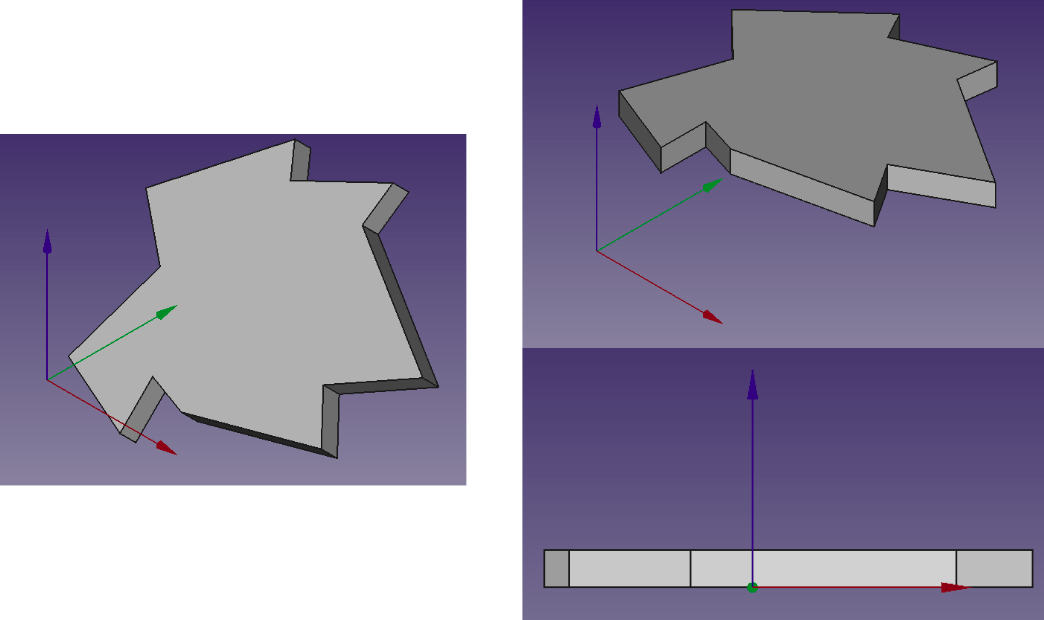
\includegraphics[scale=0.4]{Capitulos/Cap03_figs/Rotation_Face.png}
    \caption{Figura para se usar como exemplo da rotação, onde a imagem do lado esquerdo está é antes de se rotacionar, ou seja a altura não esta minimizada. Enquanto as do lado direito estão em diferentes perspectivas, para mostrar que passaram pela rotação}
    \label{fig:Cap03_FreeCad_Rotation}
\end{figure}
\subsection{Posição inicial}\label{cap:methods:initial_pos}

Após rotacionar os objetos, eles serão transladados em uma posição inicial, pois o algoritmos genético irá realizar uma translação dos objetos. Onde o vetor de translação, serão positivos em todos os eixos, logo se é interessante ter todos os vértices possuírem valores negativos em suas coordenadas.

\begin{enumerate}
    \item Realiza um \textit{loop} por todos os objetos da cena do tipo ``<class `PartDesign.Body'>" e que não possuam o nome "Board Body", pois este está reservado para a bandeja;
    \begin{enumerate}
        \item Realiza um \textit{loop} por todos os vértices;
        \begin{enumerate}
            \item Onde se verifica a coordenada dos vértices;
            \item Anotando a coordenada do maior valor de X e Y;
        \end{enumerate}
        \item Ao se determinar os maiores valores de X e Y, o objeto será transladado onde esses vértices estarão na posição zero de suas respectivas coordenadas, vide figura \ref{fig:Cap03_FreeCad_Initial_Position}.
    \end{enumerate}
\end{enumerate}

A função "\textit{Initial\_Position}" do \cite{code:FreeCad_Miner}, pode ser encontrada abaixo:

\begin{lstlisting}[language=Python, breaklines, caption = \textit{Initial\_Position}, captionpos=b]
def Initial_Position( objs ):
    #Go through every object
    for obj in objs:
        if 'Shape' in dir(obj):
            if str(type(obj)) == "<class 'PartDesign.Body'>" and obj.Label != "Board Body":
                s = obj.Shape
                p = obj.Placement
                b = p.Base
                r = p.Rotation
                #Set a realy low coordinate value on the highest at first, so it will switch for sure
                highest_x = -9999999
                highest_y = -9999999
                #Go through vetexes, looking for the highest values    
                for vertex in s.Vertexes:
                    Point = vertex.Point
                    if highest_x < Point[0]:
                        highest_x = Point[0]
                    if highest_y < Point[1]:
                        highest_y = Point[1]
                #Set new positions for object 'obj'
                obj.Placement = App.Placement(App.Vector( b[0]-highest_x, b[1]-highest_y, b[2], r) )
\end{lstlisting}

\begin{figure}[H]
    \centering
    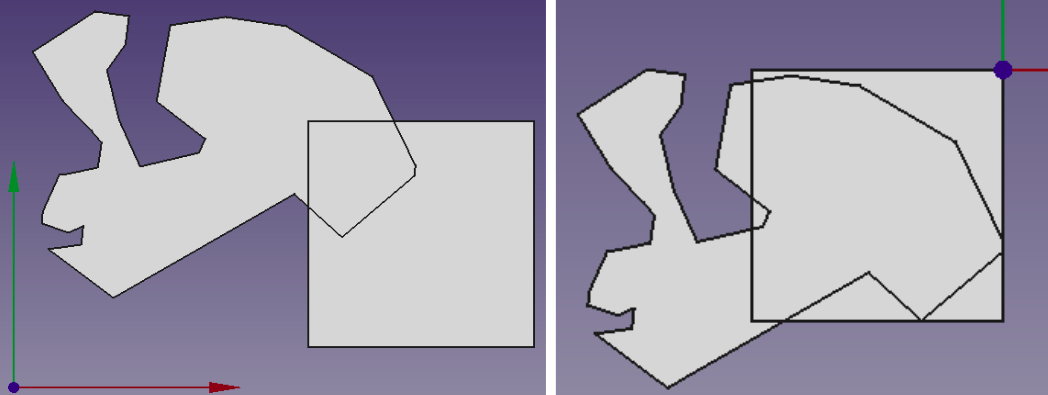
\includegraphics[scale=0.4]{Capitulos/Cap03_figs/Initial_Position.png}
    \caption{Ilustrando o resultado da função ao se rodar ela pelo \textit{FreeCad}, com a perspectiva, sendo vista de cima, para melhor mostrar o resultado da translação. Onde a imagem do lado esquerdo é a imagem da cena antes do código, e o da direita é a cena depois}
    \label{fig:Cap03_FreeCad_Initial_Position}
\end{figure}

\subsection{Coleta dos vértices}

Esse processo é necessário, devido a necessidade de se conhecer as formas dos objetos para ser possível empacota-los. Então os objetos serão processados para se coletar as coordenadas dos vértices, usando a logica abaixo:

\begin{enumerate}
    \item Realiza um \textit{loop} por todos os objetos da cena;
    \begin{enumerate}
        \item Armazena o valor da \textit{Base} dos objetos do cena, onde este é o ``centro" do objeto, não necessariamente da forma geométrica, e sim do objeto de computador. Mas devido ao fato de se reposicionar os objetos em \ref{cap:methods:initial_pos}, esse valor não é mais necessário; 
        \item Realiza um \textit{loop} por todos os vértices;
        \begin{enumerate}
            \item Anota as coordenadas X, Y e Z dos mesmos;
        \end{enumerate}
        \item Ao finalizar o processo, todas as posições e os valores das posições dos vértices estarão alocados em um lista do \textit{python}, pronto para se passar para o \textit{GA}.
    \end{enumerate}
\end{enumerate}

A função "\textit{getPositionsValues}" do \textit{script} \cite{code:FreeCad_Miner} será a responsável por esse processo:

\begin{lstlisting}[language=Python, breaklines, caption = \textit{getPositionsValues}, captionpos=b]
def getPositionsValues(objs):
    vertexesAll = []
    positions = []
    CadData = []
    for obj in objs:
        if 'Shape' in dir(obj):
            if str(type(obj)) == "<class 'PartDesign.Body'>" and obj.Label != "Board Body":
                p = obj.Placement
                b = p.Base
                #Stores position
                positions.append( [ b[ 0 ], b[ 1 ], b[ 2 ] ] )
                vertexes = obj.Shape.Vertexes
                #Object's Vertexes
                vertexes_list = []
                for vert in vertexes:
                    vertexes_list.append([vert.Point[0], vert.Point[1], vert.Point[2]])
                    
                #Vertexes for all objects
                vertexesAll.append(vertexes_list)
    return [ positions, vertexesAll ]
\end{lstlisting}

% \begin{table}[ht]
% \centering
% \begin{tabular}{c | c}
% Passo & Período Estimado \\
% \hline
% Versões de GA & Julho/Agosto \\
% Pré Processamento que acomode formas não convexas & Julho/Agosto \\
% Implementação da interface de \textit{plugins} & Julho \\
% Pós processamento & Agosto/Setembro \\
% Obtenção dos resultados & Setembro/Outubro \\
% Relatório final & Novembro
% \end{tabular}
% \caption{Cronograma de atividades}
% \label{tbl:cronograma}
% \end{table}


% \begin{code}
% \begin{minted}[frame=lines, breaklines, linenos, fontsize=\large]
% {SQL}
% SELECT last_name, department_id
%     FROM employees 
%     WHERE employee_id = 176;
% \end{minted}
% \end{code}

% \begin{lstlisting}[language=Python]
% import numpy as np
    
% def incmatrix(genl1,genl2):
%     m = len(genl1)
%     n = len(genl2)
%     M = None #to become the incidence matrix
%     VT = np.zeros((n*m,1), int)  #dummy variable
    
%     #compute the bitwise xor matrix
%     M1 = bitxormatrix(genl1)
%     M2 = np.triu(bitxormatrix(genl2),1) 

%     for i in range(m-1):
%         for j in range(i+1, m):
%             [r,c] = np.where(M2 == M1[i,j])
%             for k in range(len(r)):
%                 VT[(i)*n + r[k]] = 1;
%                 VT[(i)*n + c[k]] = 1;
%                 VT[(j)*n + r[k]] = 1;
%                 VT[(j)*n + c[k]] = 1;
                
%                 if M is None:
%                     M = np.copy(VT)
%                 else:
%                     M = np.concatenate((M, VT), 1)
                
%                 VT = np.zeros((n*m,1), int)
    
%     return M
% \end{lstlisting}

